\documentclass{article}
\usepackage[utf8]{inputenc}

% Page setup
\usepackage[a4paper,landscape,margin=2cm]{geometry}

% Typography
\usepackage[scaled]{helvet}
\let\familydefault\sfdefault

\usepackage[usenames,svgnames]{xcolor}
\usepackage{tikz}
\usetikzlibrary{positioning,arrows}

\definecolor{colorbg}  {RGB}{199,212,104}
\definecolor{colortext}{RGB}{29,29,27}

\begin{document}
\pagestyle{empty}
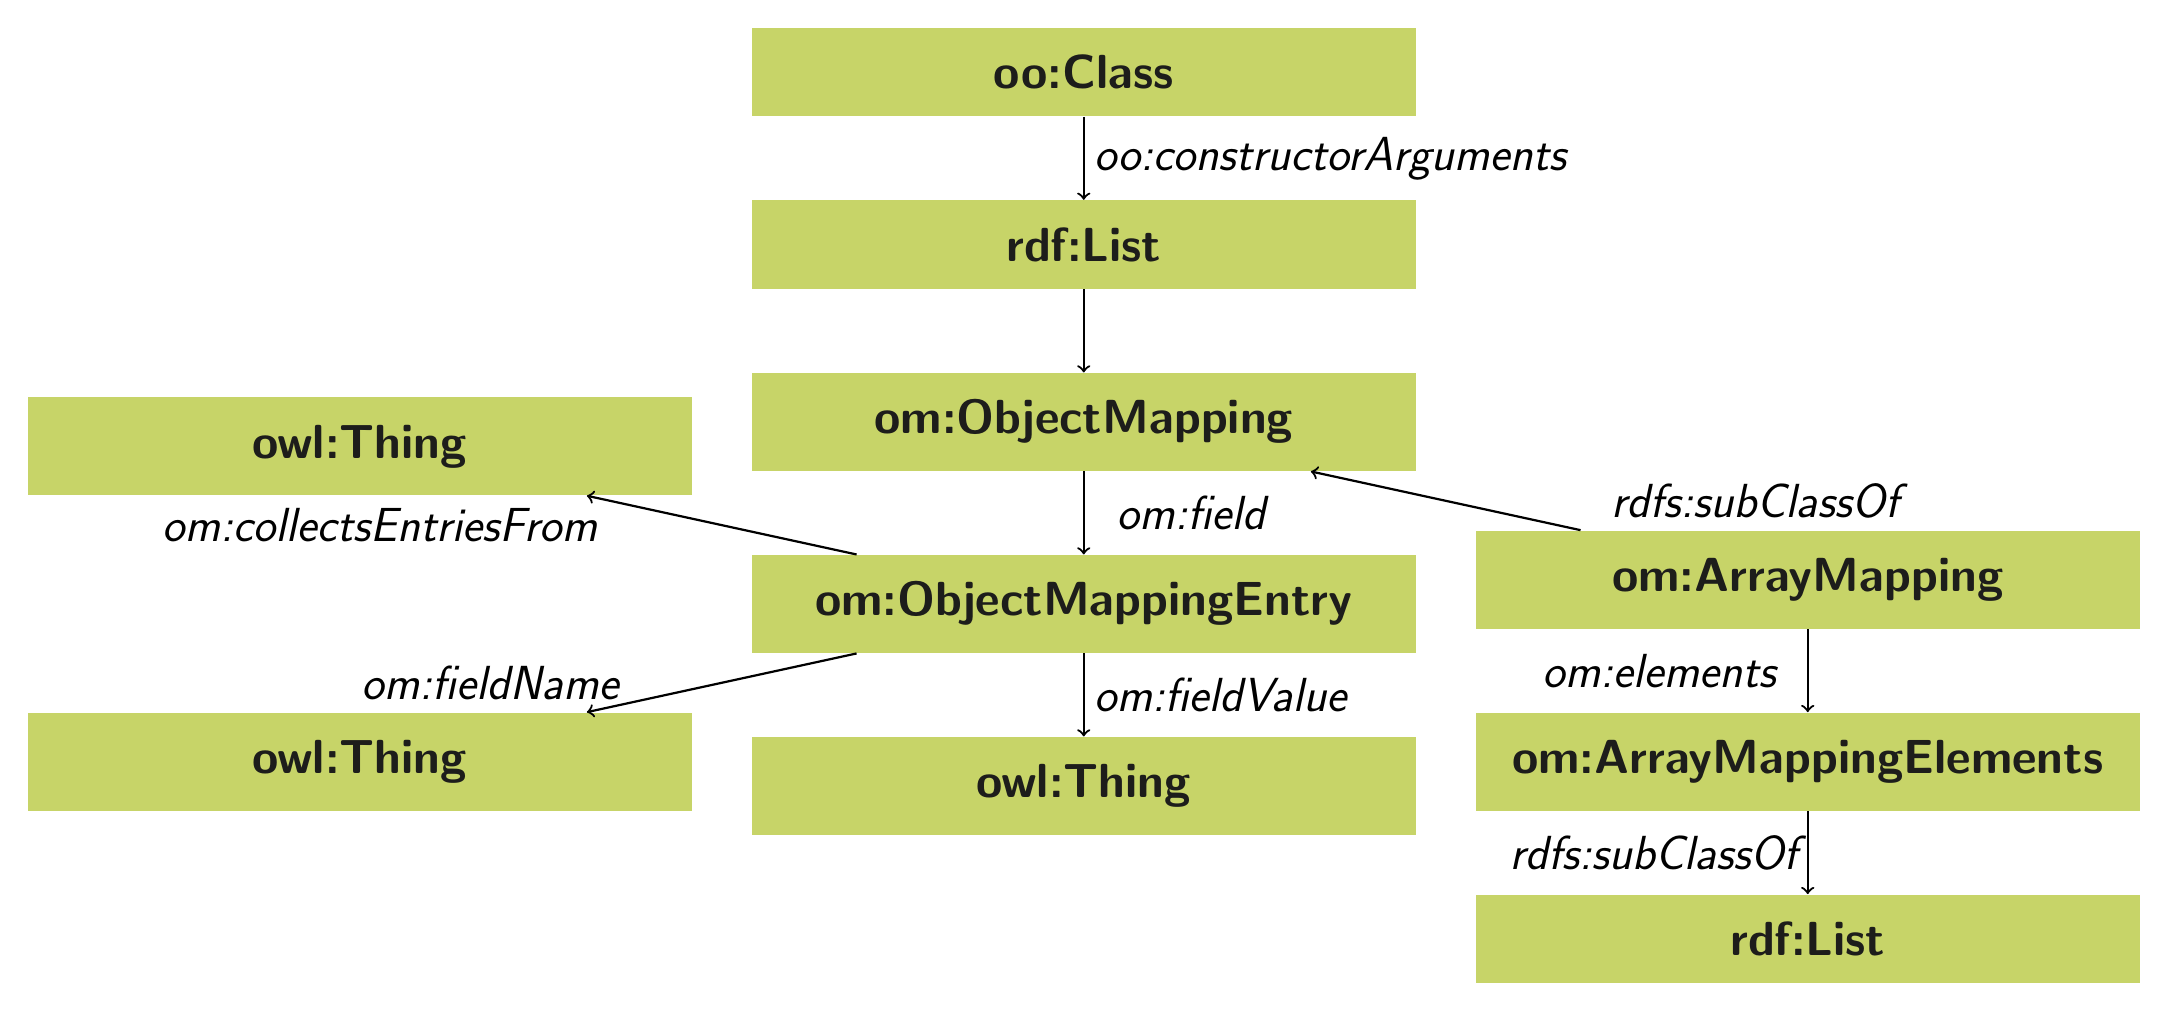
\begin{tikzpicture}[
    node distance = 3em, auto,
    font={\LARGE\itshape},
    concept/.style={text=colortext,font={\LARGE\bfseries},inner sep=10pt,align=center,rectangle,fill=colorbg,text width=22em},
    relation/.style={text width=16em},
]

    % Concepts
    \node[concept] (om)    {om:ObjectMapping};
    \node[concept, below right=of om] (am) {om:ArrayMapping};
    
    \node[concept, above=of om] (listclass) {rdf:List};
    \node[concept, above=of listclass] (class) {oo:Class};
    
    \node[concept, below=of om] (ome) {om:ObjectMappingEntry};
    \node[concept, below=of am] (ame) {om:ArrayMappingElements};
    
    \node[concept, below=of ame] (list) {rdf:List};
    
    \node[concept, below left=of ome] (name)    {owl:Thing};
    \node[concept, below=of ome] (value)    {owl:Thing};
    \node[concept, above left=of ome] (value2)    {owl:Thing};
    
    % Concept relations
    \draw[->,thick,relation,text width=17em] (class) -- (listclass) node [right,midway,align=center] {oo:constructorArguments};
    \draw[->,thick,relation,text width=17em] (listclass) -- (om) node [right,midway,align=center] {};
    
    \draw[->,thick,relation,text width=7em] (om) -- (ome) node [right,midway,align=center] {om:field};
    \draw[->,thick,relation] (am) -- (om) node [right,midway,align=right] {rdfs:subClassOf};
    
    \draw[->,thick,relation,text width=10em] (am) -- (ame) node [left,midway,align=center] {om:elements};
    \draw[->,thick,relation] (ame) -- (list) node [left,midway,align=right] {rdfs:subClassOf};
    
    \draw[->,thick,relation,text width=16em] (ome) -- (name) node [left,midway,align=center] {om:fieldName};
    \draw[->,thick,relation,,text width=8em] (ome) -- (value) node [right,midway,align=center] {om:fieldValue};
    \draw[->,thick,relation,text width=17em] (ome) -- (value2) node [left=1,midway,align=left] {om:collectsEntriesFrom};

\end{tikzpicture}
\end{document}
